In this section, we first describe two challenges in solving the traffic matrix prediction problem with partial information in Section \ref{subsection:motivation}. 
%under highly missing ground-truth data in Section \ref{subsection:motivation}. 
These two challenges then are addressed in Section \ref{subsection:data_correction} and \ref{subsection:flows_selection}, respectively.
\subsection{Motivation}
\label{subsection:motivation}
\begin{figure}
  \subfigure[10$\%$ Ground-truth input. \label{fig:lstm_prediction_10}]{
  
\includegraphics[width=.44\textwidth]{proposed_model_figs/lstm_flow_142_day_10_10.eps}
  }
  \subfigure[20$\%$ Ground-truth input.\label{fig:lstm_prediction_20}]{
  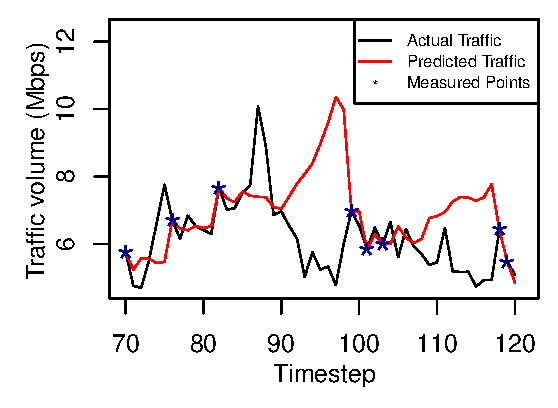
\includegraphics[width=.44\textwidth]{proposed_model_figs/lstm_flow_142_day_10_20.eps}
  }
  \subfigure[30$\%$ Ground-truth input.\label{fig:lstm_prediction_30}]{
  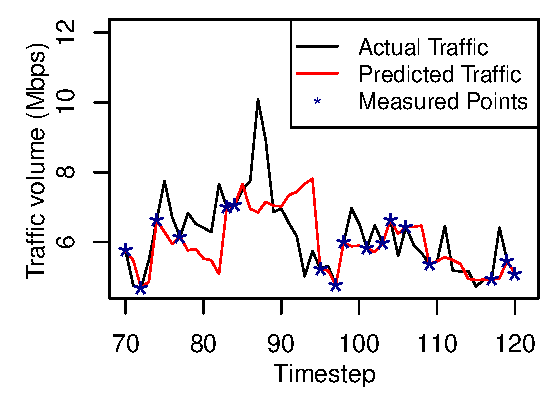
\includegraphics[width=.44\textwidth]{proposed_model_figs/lstm_flow_142_day_10_30.eps}
  }
  \subfigure[40$\%$ Ground-truth input.\label{fig:lstm_prediction_40}]{
  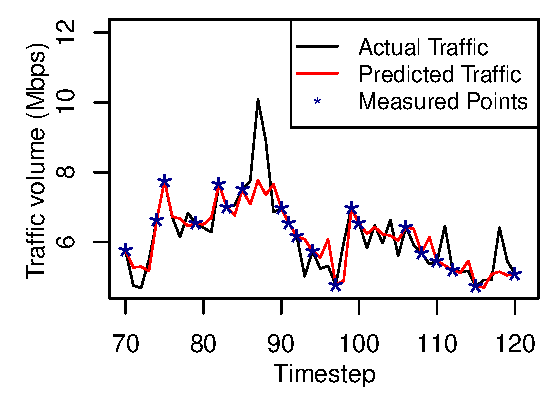
\includegraphics[width=.44\textwidth]{proposed_model_figs/lstm_flow_142_day_10_40.eps}
  }
\caption{The effect of ground-truth input on prediction accuracy. (One-step-ahead prediction using the LSTM network.)}
\label{fig:effect_ground_truth_input}
\vspace{-5pt}
\end{figure}
In order to deploy the traffic matrix prediction model, we face two important challenges. The first one is the accumulative error in the prediction results over timesteps. We have conducted an experiment to figure out the impact of imprecise input data on the results of one-step-ahead prediction (i.e., $L=1$) using the LSTM network. 
%Fig.\ref{fig:semi_recursive_pred_exp} shows the comparison between the ground-truth value and the traffic prediction results which use both precise data (obtained by direct measuring) and imprecise data (the predicted results of previous timesteps). 
Fig.\ref{fig:effect_ground_truth_input} shows the one-step-ahead prediction results with various settings of the percentage of ground-truth data in the input. As shown, the accuracy decreases over the timesteps between two consecutive measurement points (i.e., Fig.\ref{fig:lstm_prediction_10}, Fig.\ref{fig:lstm_prediction_20}). While in Fig.\ref{fig:lstm_prediction_40}, thanks to the higher percentage of ground-truth data in the input, we can capture the trend of the flow and achieve a high accuracy in forecasting the future traffic. Therefore, in order to alleviate the accumulative error while remaining the low monitoring overhead (which is proportional to the portion of the ground-truth data), our idea is to add a preprocessing on the imprecise data before feeding it into the prediction model. Specifically, we propose a novel deep learning model based on the bidirectional recurrent neural network (the details will be shown in Section \ref{subsection:data_correction}).

The second challenge is how to determine which flows to be measured at the next timestep. As mentioned above, in order to reduce the monitoring overhead we do not measure all network flows, thus choosing appropriate flows to monitor in each timestep becomes a critical factor in reducing the prediction error. One of the common approaches in choosing monitored flow set is to satisfy the fairness among all the flows. Specifically, the gaps between every two consecutive monitored timesteps of every flow are kept to be approximately the same. However, this method may not be effective since the network flows are dynamic and have various temporal fluctuation patterns. To deal with this problem, we propose a novel scheme for selecting the next monitored flows, which exploits the previous prediction results and the fluctuation characteristic of all flows (see the details in Section \ref{subsection:flows_selection}).
\subsection{Spatiotemporal traffic matrix prediction and input data correction}
\label{subsection:data_correction}
The ConvLSTM network has shown the effective capability in processing the spatial and temporal time series data where the inputs are 3D tensors such as images or video frames. 
Therefore, to apply the ConvLSTM network in our problem, we first consider the traffic matrices as 2D images with the dimension of $n \times n$, and then we transform them into 3D tensors by adding extra binary matrices (called as measurement matrices). Specifically, the measurement matrix $M_j$, which is added to the traffic matrix at timestep $j$, is a matrix whose each element $m^j_{s,d} \in M_j$ indicates whether the corresponding value in the traffic matrix is an observed value (i.e., $m^j_{s,d}=1$) or a predicted value (i.e., $m^j_{s,d}=0$). 
%Therefore, to apply the ConvLSTM network in our problem, first we consider the traffic matrices as 2D images with the dimension of $n \times n$. Then, we transform these traffic matrices to 3D tensors by adding a binary matrix $M_j$ into the traffic matrix of each timestep $j$. Specifically, $M_j$ is the measurement matrix whose each element $m^j_{s,d} \in M_j$ indicates that the corresponding value in the traffic matrix is an observed (i.e., $m^j_{s,d}=1$) or predicted value (i.e., $m^j_{s,d}=0$). Thus, we have the input of the ConvLSTM network which is a sequence of $J$ 3D tensors with the dimension of $n \times n \times 2$. 
\begin{figure}
\centering	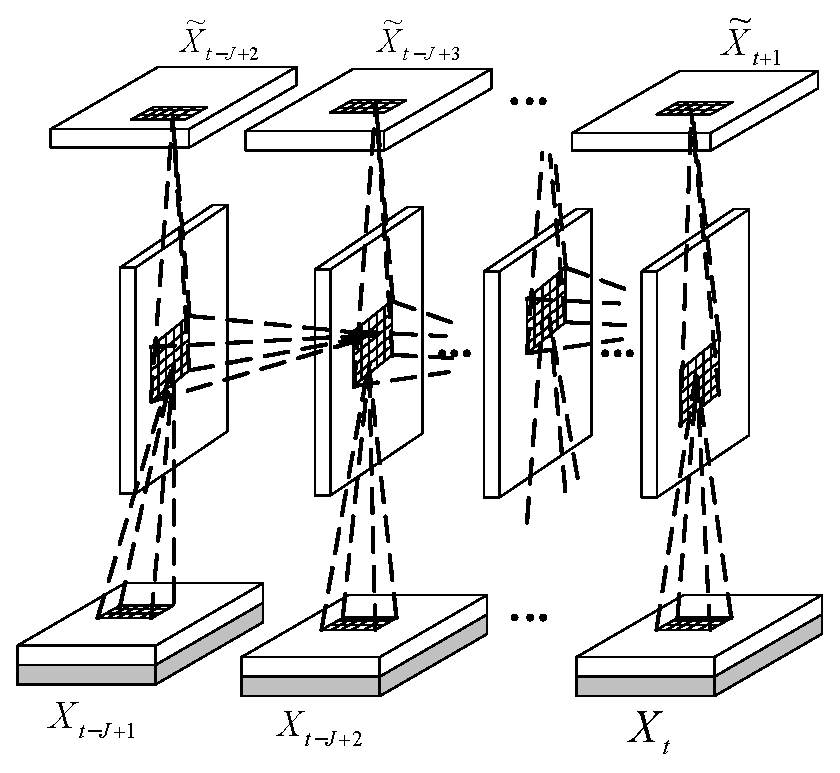
\includegraphics[width=0.6\columnwidth]{proposed_model_figs/ConvLSTM_TM_prediction.eps}
		\caption{The many-to-many model of ConvLSTM network for traffic matrix prediction. \label{fig:ConvLSTM_TM_prediction}}
        \vspace{-5pt}
\end{figure}
Thus, the input of our ConvLSTM network is a sequence of $J$ 3D tensors whose dimension is $n \times n \times 2$. 
In order to predict multi-step traffic matrices, we apply the Iterated Multi-Step estimation (IMS) approach \cite{shi2018machine}. Specifically, we first use the many-to-many model to predict the traffic matrix of the next timestep and then, iteratively feed the generated data into the model to get the multi-step-ahead prediction. Fig.\ref{fig:ConvLSTM_TM_prediction} describes the many-to-many model which takes $J$ 3D tensors from timestep $t-J+1$ to $t$ as the input and predicts the next traffic matrix $\widetilde{X}_{t+1}$. 
\begin{figure*}[bt]
\centering
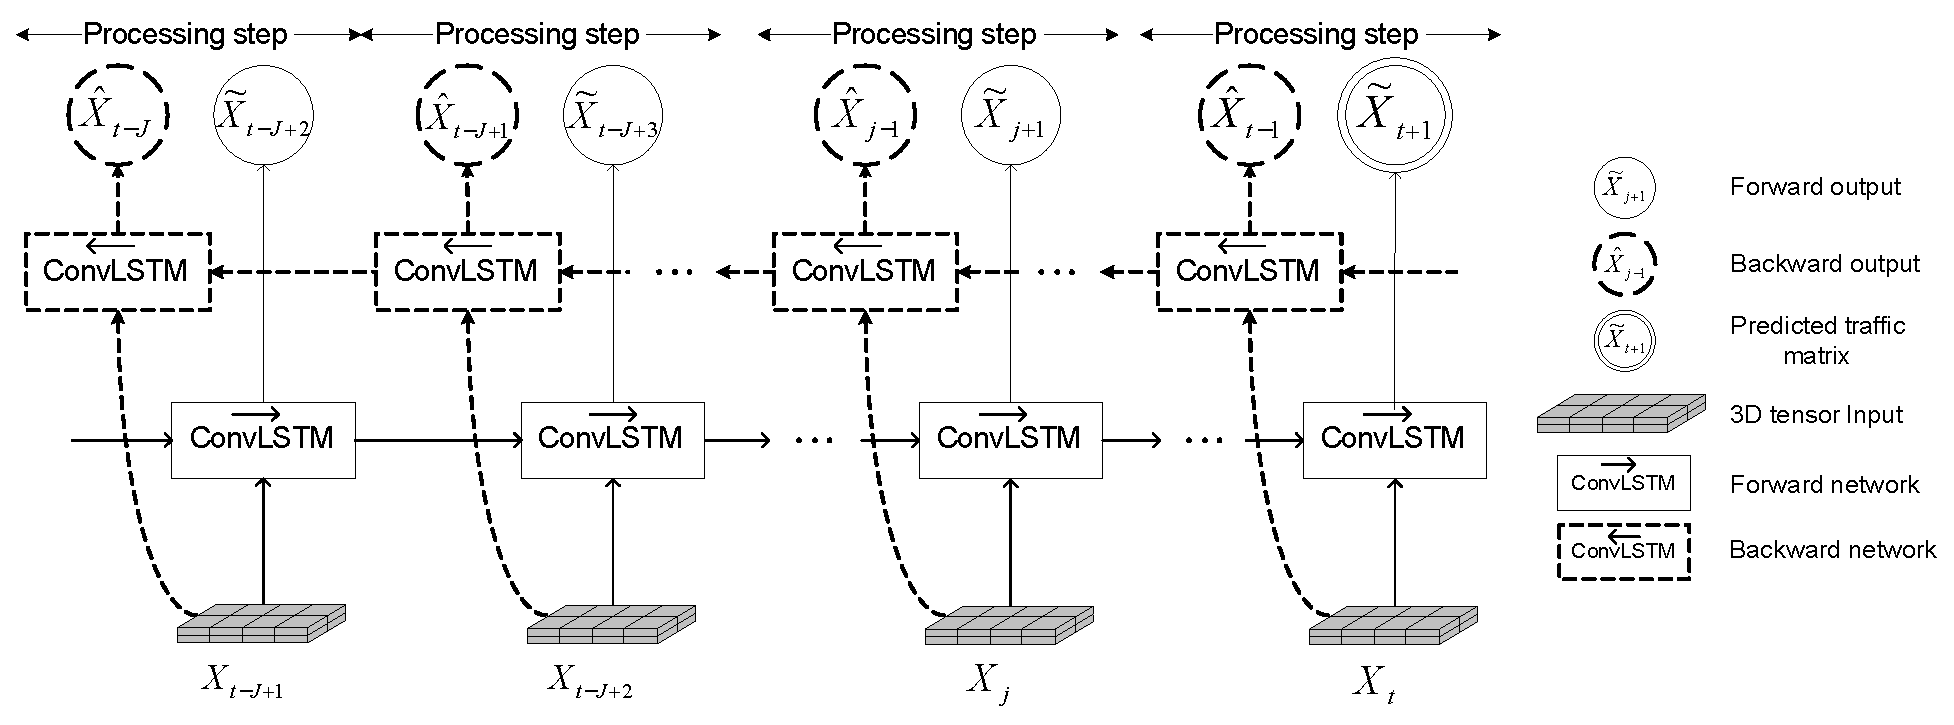
\includegraphics[width=0.65\columnwidth]{proposed_model_figs/forward_backward_model.eps}
		\caption{The forward and backward ConvLSMT networks. \label{fig:forward_backward_model}}
\end{figure*}

Now, we describe our technique for alleviating the error in the input data. Following the experiment in Section \ref{subsection:motivation} (Fig.\ref{fig:effect_ground_truth_input}), we observe that the prediction results become more accurate if the input sequence contains more precise data. Besides that, the accuracy of the predicted traffic at a timestep whose previous timestep's data is ground-truth data is better than the others. Based on the above observations, we propose an algorithm which uses the outputs from each processing step of the ConvLSTM network (i.e., $\widetilde{X}_{t-J+2},...,\widetilde{X}_{t}$) and the measurement matrices to correct the imprecise data. To be more specific, considering an example where we predict the traffic matrix $X_{t+1}$ by taking the sequence $\{X_{t-J+1},...,X_t\}$ as the input. As using the many-to-many model, after the prediction, we also obtain the outputs $\{\widetilde{X}_{t-J+2},...,\widetilde{X}_{t+1}\}$ whose each element corresponds to one processing step of the ConvLSTM network. Suppose that $x_{s,d}^j \in X_j$ ($t-J+2 \leq j \leq t$) is an imprecise data and $\widetilde{x}^j_{s,d} \in \widetilde{X}_{j}$ is its corresponding output in the ConvLSTM network. Because of the forward direction in the processing step of the ConvLSTM network, the output $\widetilde{x}^j_{s,d}$ is generated by taking only the input from timestep $t-J+1$ to $j-1$. If the input sequence from timestep $t-J+1$ to $j-1$ contains almost ground-truth data, we can replace $x_{s,d}^j$ by $\widetilde{x}^j_{s,d}$. However, we face with the problem when the input sequence from timestep $t-J+1$ to $j-1$ contains only a few ground-truth data. To this end, our idea is to leverage the data at the next timesteps (from $j+1$ to $t$) which may include more precise data.

In order to implement the above idea, besides the current ConvLSTM network (which we call as the \textit{forward network}), we construct an extra network (called as the \textit{backward network}) in which the input data is fed in the reverse order. 
Our approach is motivated by the Bidirectional Recurrent Neural Network (BRNN) which was introduced in \cite{schuster1997bidirectional}. Thanks to adding a backward network, BRNN can be trained by all available input information in both the past and the future of a specific time frame. Different from the standard BRNN, in each processing step, instead of aggregating the outputs of the forward and backward networks, we keep them separately (as shown in Fig.\ref{fig:forward_backward_model}), and use the outputs from the backward network to update the incorrect data in the input matrices. Therefore, $x_{s,d}^j$ now can be updated by using the output of the forward network (i.e., $\widetilde{x}^j_{s,d}$) or the output of the backward network (i.e., $\widehat{x}^j_{s,d}$). 
In order to determine the contribution of the old value (i.e., $x_{s,d}^j$), the outputs of the forward and backward networks (i.e., $\widetilde{x}^j_{s,d}$ and $\widehat{x}^j_{s,d}$) in updating imprecise data, we define parameters $\alpha_{s,d,t}$, $\beta^j_{s,d,t}$ and $\gamma^j_{s,d,t}$ which are the confidence factors of $x_{s,d}^j$, $\widetilde{x}_{s,d}^j$ and $\widehat{x}_{s,d}^j$, respectively ($\alpha_{s,d,t} + \beta^j_{s,d,t} + \gamma^j_{s,d,t} = 1$). The details of the imprecise data correction algorithm is described in Algorithm \ref{algo:data_correction}. Note that since the outputs of the forward network are from timestep $t-J+2$ to $t+1$ while that of the backward network are from $t-J$ to $t-1$, we can only apply Algorithm \ref{algo:data_correction} for correcting the inputs from timestep $t-J+2$ to $t-1$. In what follows, we describe the main idea behind Algorithm \ref{algo:data_correction}. 
\begin{algorithm}[bt]
%\begin{algorithmic}[1]
\SetAlgoLined
\Input{
$X_k$: the previous traffic matrix at timestep $k$ \newline
$\widetilde{X}_k$: the outputs of forward network \newline
$\widehat{X}_k$: the outputs of backward network \newline
$M_k$: the measurement matrix of $X_k$ \newline
($k = t-J+2,...,t-1$)}
\Output{The updated traffic matrices}
\For{$ s, d \in \mathcal{N}$}{
	$\alpha_{s,d,t} \leftarrow 1 - \frac{\sum_{i=t-J+1}^{t}{m^i_{s,d,t}}}{J}$ \;
	\If{$(\sum_{i=t-J+1}^{t}m^i_{s,d} \neq 0)$}{
        $l_{s,d,t}^f \leftarrow \sqrt{\sum_{j=t-J + 2}^{t-1}		{m_{s,d}^j\times(\widetilde{x}_{s,d}^j - x_{s,d}^j)^2}}$\;
       $l_{s,d,t}^b \leftarrow \sqrt{\sum_{j=t-J + 2}^{t-1}{m_{s,d}^j\times(\widehat{x}_{s,d}^j - x_{s,d}^j)^2}}$\;
    }
    \Else{
    	$l_{s,d,t}^f \leftarrow \xi$; \quad $l_{s,d,t}^b \leftarrow \xi$ \;
    }
    \For{$j=t-J+2$ \textbf{to} $t-1$}{
    	$\rho^j_{s,d,t} \leftarrow \frac{\sum_{i=t-J+1}^{j-1}{m^i_{s,d,t}}}{j - t + J}$; \quad
        $\mu^j_{s,d,t} \leftarrow \frac{\sum_{i=j+1}^{t}{m^i_{s,d,t}}}{t - j}$ \;
		$\beta^j_{s,d,t} \leftarrow \frac{(l_{s,d,t}^b + \rho^j_{s,d,t})(1 - \alpha_{s,d,t})}{l_{s,d,t}^f + l_{s,d,t}^b + \rho^j_{s,d,t} + \mu^j_{s,d,t}}$ \;
		$\gamma^j_{s,d,t} \leftarrow \frac{(l_{s,d,t}^f + \mu^j_{s,d,t})(1 - \alpha_{s,d,t})}{l_{s,d,t}^f + l_{s,d,t}^b + \rho^j_{s,d,t} + \mu^j_{s,d,t}}$\;
        $x_{s,d}^j \leftarrow \alpha_{s,d,t} \times x_{s,d}^j  + \beta^j_{s,d,t} \times \widetilde{x}_{s,d}^j + \gamma^j_{s,d,t} \times \widehat{x}_{s,d}^j$\;
    }
}
\Return $X_k$ ($k = t-J+2,...,t-1$)
\caption{\label{algo:data_correction}\footnotesize{Forward and backward data correction}}
%\end{algorithmic}
\end{algorithm}

Obviously, the less the ground-truth data contained in the inputs, the less precise the predicted values, thus $x_{s,d}^j$ should not be updated if the historical data is highly missed. Accordingly, the confidence factor $\alpha_{s,d,t}$ in Algorithm 1 is determined by the portion of the flows that are not monitored (line 2).  
%designed to be proportional to the ratio of the missed historical data in the input sequence (line 2). 
%In Algorithm \ref{algo:data_correction}, first, the confidence factor $\alpha_{s,d,t}$ is assigned to be equal the missing ground-truth ratio in the input of flow ($s,d$) since $x_{s,d}^j$ should be remained when the input sequence has high missing ground-truth data ($\alpha_{s,d,t} \approx 1$). 
%We discuss more details about $\beta^j_{s,d,t}$ and $\gamma^j_{s,d,t}$ by first introducing two terms \textit{forward loss} and \textit{backward loss}.
$\beta^j_{s,d,t}$ and $\gamma^j_{s,d,t}$ are determined based on two terms named \textit{forward loss} and \textit{backward loss}.
The forward and backward losses of a flow $(s,d)$ (denoted as $l_{s,d,t}^f$ and $l_{s,d,t}^b$, respectively) are defined to assess the performance of the forward and backward ConvLSTM networks after predicting the traffic at current timestep $t$. Specifically, $l_{s,d,t}^f$ and $l_{s,d,t}^b$ are defined as the root squared errors between the outputs and the ground-truth elements in the input (line 4, 5). Note that, if the input contains no ground-truth data, then the losses are assigned to $\xi$ which is a very large positive number (line 8).
Intuitively, the smaller $l_{s,d,t}^f$ (resp. $l_{s,d,t}^b$), the smaller the gap between $\widetilde{x}_{s,d}^j$ (resp. $\widehat{x}_{s,d}^j$) and the ground-truth. Therefore, if $l_{s,d,t}^f < l_{s,d,t}^b$, then $\widetilde{x}_{s,d}^j$ should contribute more than $\widehat{x}_{s,d}^j$ in correcting the imprecise input, otherwise, $\widehat{x}_{s,d}^j$ should contribute more than $\widetilde{x}_{s,d}^j$.
Accordingly, the confidence factors $\beta^j_{s,d,t}$ is designed so that flows with the small $l_{s,d,t}^f$ and the large $l_{s,d,t}^b$ will have the large $\beta^j_{s,d,t}$. 
%to be inversely proportional to $l_{s,d,t}^f$ and proportional to $l_{s,d,t}^b$. 
Inversely, flows with the small $l_{s,d,t}^b$ and the large $l_{s,d,t}^f$ will have the large $\gamma^j_{s,d,t}$.
%$\gamma^j_{s,d,t}$ is inversely proportional to $l_{s,d,t}^b$ and proportional to $l_{s,d,t}^f$. 
%Obviously $\widetilde{x}_{s,d}^j$ should contribute in the corrected result more than $\widehat{x}_{s,d}^j$ if $l_{s,d,t}^f$ is lower than the $l_{s,d,t}^b$ and otherwise. Therefore, the confidence factors $\beta^j_{s,d,t}$ and $\gamma^j_{s,d,t}$ are invert proportional with the forward and backward loss. 
Moreover, with the observation that the more ground-truth elements the inputs contain, the more accurate the prediction result is, $\beta^j_{s,d,t}$ (resp. $\gamma^j_{s,d,t}$) is also designed so that the greater the percentage of the ground-truth data in the input at timesteps from $t - J + 1$ to $j - 1$, i.e., denoted as $\rho^j_{s,d,t}$ (resp. from $j + 1$ to $t$, i.e., denoted as $\mu^j_{s,d,t}$), the greater the $\beta^j_{s,d,t}$. Consequently, $\beta^j_{s,d,t}$ and $\gamma^j_{s,d,t}$ are calculated based on both the network losses and the percentage of ground-truth data in the input (line 12, 13). Finally, $x^j_{s,d}$ is updated by the formulation described in line 14.
\begin{figure*}
\centering
	\subfigure[ARIMA
    \label{fig:prediction_result_arima}]{
    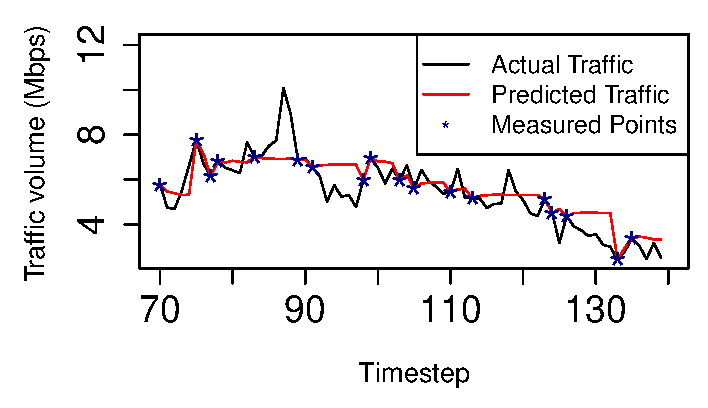
\includegraphics[width=0.28\columnwidth]{evaluation_figs/arima_flow_142_day_10.eps}  
    }
    \hfill
    \subfigure[The LSTM network
    \label{fig:prediction_result_lstm}]{
\includegraphics[width=0.28\columnwidth]{evaluation_figs/lstm_flow_142_day_10.eps}
    }
      \hfill
    \subfigure[Our proposal
    \label{fig:prediction_result_our}]{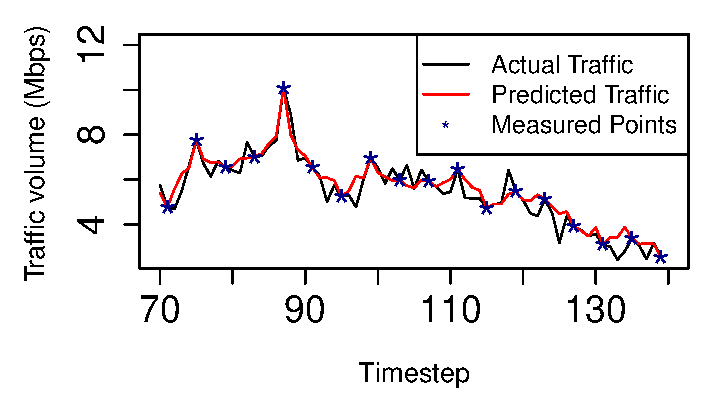
\includegraphics[width=0.28\columnwidth]{evaluation_figs/cnn_brnn_flow_11_10_day_10.eps}
    }
    \vspace{-10pt}
	\caption{Prediction results and actual values of a random flow.} 
    \label{fig:prediction_result}
\end{figure*}
\subsection{Determining the monitored flow set}
\label{subsection:flows_selection}
Our main idea is that at each timestep $t$, we calculate a weight $w_{s,d,t}$ for each flow $(s, d)$ and choose at most $k$ flows which have the lowest weights to monitor at the next timestep (i.e., timestep $t+1$). The maximum number of flows that can be monitored (i.e., $k$) depends on the network monitoring policy. In the following, before going to the details of the weight's formula, we will first describe our theoretical basis. To ease the presentation, we call the periods between the consecutive measured timesteps of a flow as non-monitored periods of that flow.

Following the experiment results shown in Section \ref{subsection:motivation}, we note that the longer the non-monitored periods, the larger the difference between the predicted results and the actual traffic. Thus, in order to reduce the prediction error, we should decrease the non-monitored periods of all flows. More specifically, the flows that have not been monitored for a long period should be chosen to be monitored at the next timestep. To this end, for each flow $(s,d)$, we define a term named \textit{consecutive missing} (denoted as $c_{s,d,t}$) which is the number of the timesteps from when $(s,d)$ was last monitored till the current timestep $t$. The weight should be designed so that it will decline when the consecutive missing gets high.

Moreover, since our imprecise data correction algorithm is based on the outputs of the forward and backward networks, we need to keep the losses of these networks (i.e., $l^f_{s,d,t}$ and $l^b_{s,d,t}$, respectively) as smaller as possible. Accordingly, the flows with higher forward and backward losses should be chosen to be monitored at the next timestep.
%since our imprecise data correction algorithm is based on the forward and backward losses (defined in Section \ref{subsection:data_correction}), the algorithm may perform well in correcting the imprecise data of flows whose losses are lower than the others. Therefore, in order to alleviate this accumulative error, the flows with high backward loss and forward loss should be chosen to be monitored at the next timestep.

Finally, we see that the flows with high fluctuation tend to have high prediction error. Therefore, these flows should be monitored more frequently. In order to measure the unsteadiness of flow $(s,d)$, we use the standard deviation of the traffic volume of the flow $(s,t)$ from timestep $t-J+1$ to $t$ (denoted as $\eta_{s,d,t}$). 

Consequently, the weight is calculated based on the flows' consecutive missing, backward loss, forward loss, and fluctuation as follows.
\begin{equation}
\label{eq_flow_weight}
\begin{aligned}
&w_{s,d,t} \\
& \ = \frac{1}{\lambda_1 \times l^f_{s,d,t} + \lambda_2 \times l^b_{s,d,t} + \lambda_3 \times c_{s,d,t} + \lambda_4 \times \eta_{s,d,t}}
\end{aligned}
\end{equation}
where $\lambda_1$, $\lambda_2$, $\lambda_3$ and $\lambda_4$ are hyper-parameters which are chosen by experiments.  

At the end of the timestep $t$, the weights of all flows are calculated, and the first $k$ flows with the lowest weights are chosen to be measured at the next timestep (i.e., timestep $t+1$).
%($d$ is the maximum number of flows can be measured depend on the network monitoring policy).
% \begin{figure}
% \RawFloats
% \begin{minipage}{0.45\textwidth}
% 	\centering
% 	\includegraphics[width=1\columnwidth]{preliminaries_figs/definitions.eps}
% 	\caption{Illustration of definitions. \label{fig:def}}
% \end{minipage}
% \hfill
% \begin{minipage}{0.45\textwidth}
% 	\centering
% 		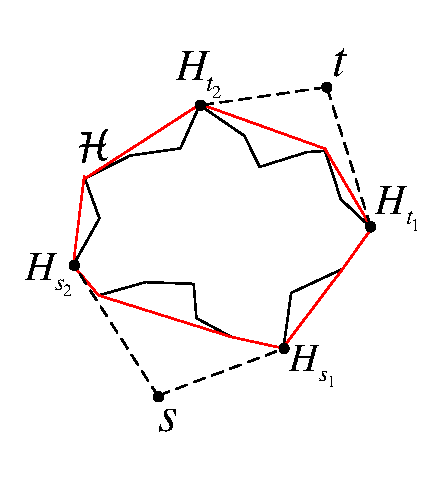
\includegraphics[width=0.8\columnwidth]{motivation_figs/shortest_path.eps}
% 		\caption{Illustration of Proposition \ref{pro:shortest_path}. \label{fig:pro_shortest_path}}
% \end{minipage}
% \end{figure}